%  
%  信号処理シンポジウム (SIPS) 用テンプレート
%
\documentclass[10pt,japanese]{ikelab-sips}

% Times フォントに変更
% (LaTeX のデフォルトフォントがちょっと見づらいと感じるなら)
%\usepackage{newtxtext}

% fleqn オプションを入れないとデフォルトの左寄せ設定が壊れる
\usepackage[cmex10,fleqn]{amsmath}
\usepackage{amssymb,amsfonts,latexsym,mathtools,bm}
\usepackage[dvipdfmx]{graphicx}

\usepackage{cite}
% SIPS の指定フォーマットに修正 ([1]-[3])
\renewcommand{\citeleft}{}
\renewcommand{\citeright}{}
\renewcommand{\citepunct}{, }
\renewcommand{\citedash}{--}
\renewcommand{\citeform}[1]{[#1]}

% [label=quad] で jarticle の仕様に合わせる
\usepackage[compatibility=false,labelsep=quad]{caption}
\usepackage{subcaption}

\usepackage{algorithm,algorithmic}

% argmin
\DeclareMathOperator*{\argmin}{argmin}

\jtitle{信号処理シンポジウム}

\etitle{Signal Processing Symposium}

\jauthor{
  通信一郎$^{\dag}$ \hspace{2cm}
  信号太郎$^{\ddag}$
}

\eauthor{
  Ichiro TSUSHIN$^{\dag}$ \hspace{2cm}
  Taro SHINGO$^{\ddag}$
}

\jaddress{
  \dag 電子大学工学部 \\
  \ddag (株) 電子システム研究所
}

\eaddress{
  \dag Denshi University \\
  \ddag Denshi Corp.
}

\begin{document}
\maketitle

\begin{abstract}
   % ここに 300 字程度でアブストラクトを書いてください.
   SIP Symposium 日本語用テンプレート.
  In this paper, we propose an example-based single image super resolution (SR) method by $\ell_2$
  approximation with self-sampled image patches.
  Example-based super resolution methods can reconstruct high resolution image patches
  by linear combination of atoms in overcomplete dictionary.
  This reconstruction requires a pair of two dictionaries created
  by tremendous low and high resolution image pairs
  from the prepared image databases.
  In our method, we introduce the dictionary by random sampling patches
  from only an input image without training.
  This dictionary exploits self-similarity of images and
  it will no more depend on external image set in regard to storage space
  or the accuracy of referred image set.
  In addition, we modified the approximation of
  input image to $\ell_2$ norm minimization problem, instead of commonly used
  sparse approximation such as $\ell_1$ norm regularization.
  The $\ell_2$ approximation has an advantage of computational cost
  by only solving inverse problem.
  Through some experiments, the proposed method drastically reduces the computational time for SR,
  and provides comparable performance to conventional example-based SR methods
  with $\ell_1$ approximation and dictionary training.
\end{abstract}

\section{Example-based Super Resolution} \label{sec:ebsr}
\renewcommand{\l}{\left}
\renewcommand{\r}{\right}
\newcommand{\asVector}[1]{\expandafter\def\csname #1\endcsname{{\bm{#1}}}}
\asVector{X}
\asVector{Y}
\asVector{D}
\asVector{F}
\asVector{I}
\asVector{x}
\asVector{y}
\asVector{f}
\renewcommand{\a}{\bm{\alpha}}
Example-based SR algorithms deal with this problem by representing
the LR image patch as combination of image patches and adding
the regularizer to this combination coefficients.
\cite{IEEEexample:conf_typical,IEEEexample:article_typical},
We describe one
$\sqrt{n}\times\sqrt{n}$
patch of HR image as a vector
replesented by $\bm{x}\in\mathbb{R}^{n}$.
This patch $\x$ can be combinated by
HR patch dictionary of $K$ atoms $\bm{D}_{h}\in\mathbb{R}^{n \times K}$
and its coefficient vector $\bm{\alpha} \in \mathbb{R}^{K}$
shown as follow: %\cite{Yang2008}
%
\begin{align}
 \x=\D_h\a\label{eq:X=DHa}
\end{align}
%
The relation (\ref{eq:X=DHa}) is applied similary
for representing the LR patch $\bm{y}$ which came from whole LR image $\bm{Y}$
using the LR patch dictionary $\bm{D}_{l}$ and its coefficient vector $\a$:
%
\begin{align}
 \y=\D_l\a.
\end{align}
%
Note that both two trained dictionaries $\bm{D}_{h}$ and $\bm{D}_{l}$ have
the same representation $\bm{\alpha}$ for a certain image patch.
In order to make this problem be well-posed, the sparse constraint is often imposed
by $\ell_0$ norm of $\a$ shown as follows \cite{Yang2008,Yang2010}:
%
\begin{align}
\x = \D_h\a\qquad\mathrm{with}\quad\|\a\|_0 \ll K.
\label{eq:X=DHa_sparse}
\end{align}
%

\subsection{Self-sampled Dictionaries}\label{sec:self-sampled}
%
\begin{figure}[t]
 \centering
 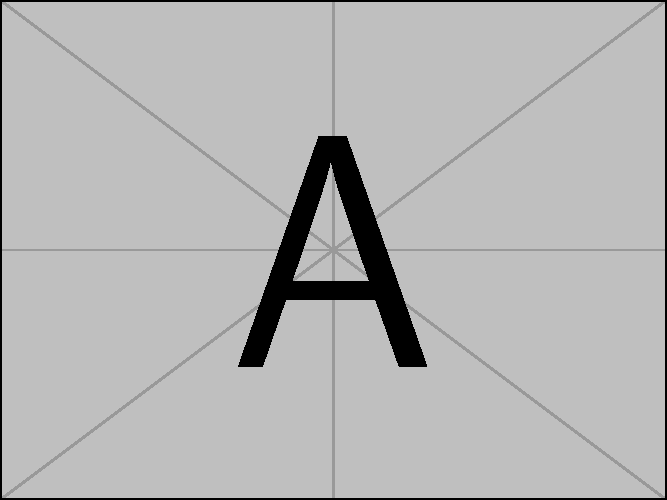
\includegraphics[width=0.8\hsize]{example-image-a.pdf}
\caption{Dictionary generation phase of proposed method}
\label{fig:sd_dic}
\end{figure}

\begin{figure}[t]
 \centering
 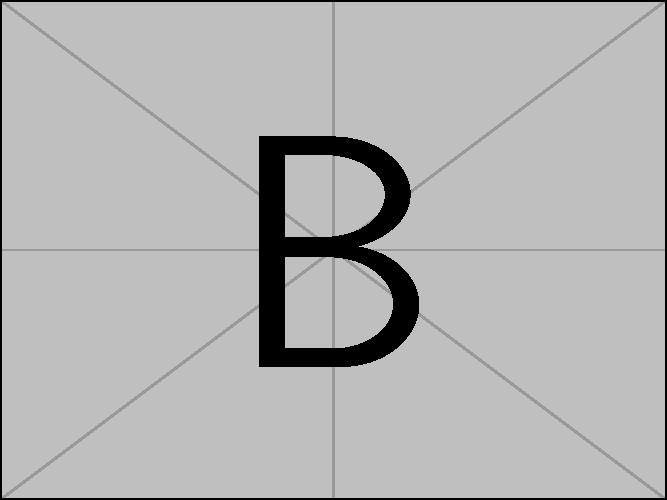
\includegraphics[width=0.9\hsize]{example-image-b.pdf}
\caption{SR reconstruction phase of proposed method}
\label{fig:sd_sr}
\end{figure}

In order to reconstruct the HR image $\X$, the pair of LR and HR dictionaries $\D_l, \D_h$ will be required.
These dictionaries are usually generated from external training examples.
In natural images, similar patches often appear not only in the
image but also in its different scale images \cite{Glasner2009}.
Based on this property, we produce LR and HR dictionaries from the input image $\Y$ alone.


\subsection{HR patch reconstuction}

 \begin{algorithm}[t]
  \caption{HR patch reconstruction process in \cite{Yang2012}} \label{algo:prev}
  \begin{algorithmic}[1]
   \FOR{each LR patch $\y\in\mathbb{R}^{n\times 1}$ in $\Y$}
   \STATE Set $m\leftarrow\mathrm{mean}(\y)$ as a DC component of $\y$ and,
   \STATE reduce the DC component from LR patch $\y\coloneqq\y-m\bm{1}$;
   \STATE Set $r\leftarrow\|\y\|_2$ as the norm of LR patch (before feature extraction;)
   \STATE Extract gradient feature $\hat\y\coloneqq\F\y$ for $\y$;
   \STATE Normalize the gradient feature $\hat\y\coloneqq\hat\y/\|\hat\y\|_2$;
   \STATE Estimate the dictionary coefficients $\a$ (by $\ell_1$ minimization, eq.\,\ref{eq:getalpha_l1};)
   \STATE Recover HR patch feature $\hat\x=\D_x\a$;
   \STATE Recover HR patch by adjusting its norm to LR patch's one: \\
   $\x\coloneqq (c \times r / \|\hat\x\|_2) \hat\x + m\bm{1}$\quad ($c$ is emperically set constant);
   \STATE Add $\x$ to the corresponding pixels in HR image $\X$
   \ENDFOR
  \end{algorithmic}
 \end{algorithm}

 \begin{algorithm}[t]
  \caption{Modified HR patch reconstruction process} \label{algo:prop}
  \begin{algorithmic}[1]
   \FOR{each LR patch $\y\in\mathbb{R}^{n\times 1}$ in $\Y$}
   \STATE Set $m\leftarrow \mathrm{mean}(\y)$ as a DC component of $\y$ and,
   \STATE reduce the DC component from LR patch $\y\coloneqq\y-m\bm{1}$;
   \STATE Extract gradient feature $\hat\y\coloneqq\F\y$ for $\y$;
   \STATE (Not normalizing the gradient feature $\hat\y$,) \\
   estimate the dictionary coefficients $\a$ (by $\ell_2$ minimization, eq.\,\ref{eq:getalpha};)
   \STATE Recover HR patch feature $\hat\x=\D_x\a$;
   \STATE Recover HR patch by adding DC component $\x\coloneqq\hat\x+m\bm{1}$, \\
   (not scaling the dynamic range of HR patch feature;)
   \STATE Add $\x$ to the corresponding pixels in HR image $\X$
   \ENDFOR
  \end{algorithmic}
 \end{algorithm}

 With the optimal solution $\bm{\alpha}$ from (\ref{eq:getalpha}),
 the HR patch feature can be estimated by $\hat\x=\D_h\alpha$.
 We modified the process to recover HR patch $\x$ from its feature $\hat\x$
 from $\ell_1$-based recovering refered in \cite{Yang2012}.
 The procedure with $\ell_1$ recovery is shown in Algorithm \ref{algo:prev} and
 the modified procedure is in Algorithm \ref{algo:prop}.
 Each process reduces the DC component $m$ of LR patch $\y$.
 This is because the feature extractive operation $\F$ cuts down the DC component of
 input patches $\y$, and the coefficient $\a$ doesn't contain the information of the DC component
 in LR or HR patches.

\section{Experimental results} \label{sec:experiments}

In order to evaluate our image reconstruction framework,
we conduct some experiments on 31 standard test images
and apply the proposed SR method using $\ell_2$ approximation.
The size of all test images are $512\times 512$,
and we enlarged these images by factor 2 using SR algorithms,
after shrinking manually by factor 2.
In addition to our SR algorithm,
general bicubic interpolation algorithm and
$\ell_1$ minimization SR algorithm
refered in Section. \ref{sec:ebsr} are evaluated for comparison.
The differences between our algorithm and $\ell_1$-based algorithm consist of two parts,
$\ell_2$-based minimization and self-sampled dictionary.
Therefore we additionally evaluated the algorithms 
including one of our new-points, namely,
algorithm using $\ell_2$-based minimization with prepared dictionary and
algorithm using $\ell_1$-based minimization with self-sampled dictionary.

\newcommand{\resultfig}[4]{
\begin{minipage}[t]{.22\hsize}
 \centering
 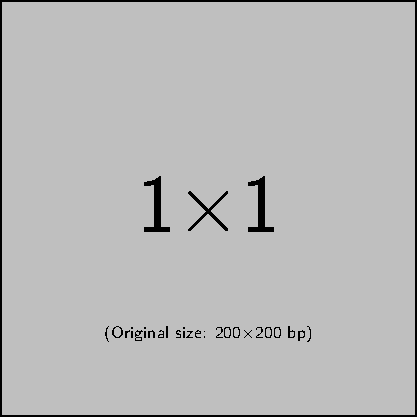
\includegraphics[width=0.9\hsize]{example-image-1x1.pdf}
 \subcaption{#3\\($\mathrm{PSNR}=#4\,\mathrm{dB}$)}\label{fig:#1:#2}
\end{minipage}
}

\newcommand{\resultfigWithoutPsnr}[3]{
\begin{minipage}[t]{.22\hsize}
 \centering
 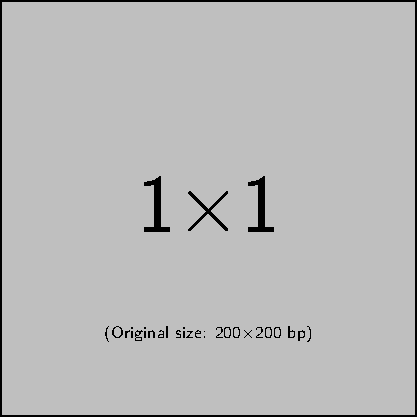
\includegraphics[width=0.9\hsize]{example-image-1x1.pdf}
 \subcaption{#3\\{}}\label{fig:#1:#2}
\end{minipage}
}

\newcommand{\resultdata}[1]{\relax}
\newcommand{\defineresultdata}[5]%
{\renewcommand{\resultdata}[1]{\ifcase##1\or{#1}\or{#2}\or{#3}\or{#4}\or{#5}\fi}}

%%% Airplane %%%
%\row{2}{Airplane}{30.869}{33.875}{33.756}{33.481}{33.791}
\defineresultdata{30.869}{33.875}{33.756}{33.481}{33.791}
\begin{figure*}[t]
 \centering
 \resultfigWithoutPsnr{airplane}{airplane}{Original $512\times 512$ Image}
 \resultfigWithoutPsnr{airplane}{gnd}{Ground-truth HR}
 \resultfigWithoutPsnr{airplane}{lr}{Input LR Image}
 \resultfig{airplane}{bic}{Bicubic}{\resultdata{1}}
 \resultfig{airplane}{pre_l1}{Predefined dictionary ($\ell_1$)}{\resultdata{2}}
 \resultfig{airplane}{pre_l2}{Predefined dictionary ($\ell_2$)}{\resultdata{3}}
 \resultfig{airplane}{self_l1}{Self-sampled dictionary ($\ell_1$)}{\resultdata{4}}
 \resultfig{airplane}{self_l2}{Self-sampled dictionary ($\ell_2$)}{\resultdata{5}}
 \caption{Experimental result in Image ``Airplane'', compareing the letter part of size $64\times 64$.}
 \label{fig:result_airplane}
\end{figure*}


  
\begin{table*}[t]
% 内訳を書くくらいなら棒グラフにでもしたほうがいいかもしれない
\def\m#1#2#3{\multicolumn{#1}{#2}{#3}}
\def\cl{\cline{2-5}}
\centering
\caption{%
Execution time compareing bicubic, $\ell_1$, $\ell_2$ algorithms with prepared dictionary and
self-sampled dictionary. Execution time of each algorithm steps are also shown in example-based algorithms.
}
\label{table:exectime}
\begin{tabular}{|l|c|c|c|c|}
 \hline
&\m{4}{c|}{Execution time (second)} \\\cl
&\m{2}{c|}{Prepared} & \m{2}{c|}{Self-sampled} \\\cl
& \makebox[8ex][c]{L1} & \makebox[8ex][c]{L2} & \makebox[8ex][c]{L1} & \makebox[8ex][c]{L2} \\\hline
Whole execution time 
&  7.932 & \textbf{0.541} &   3.462  & 1.163 \\\hline
--- with dictionary preparation   
&   $-$  &      $-$       &   0.633  & 0.631 \\
--- with inverse matrix operation 
&   $-$  &     0.026      &    $-$   & 0.025 \\
--- with optimization  
&  7.494 &     0.073      &   2.390  & 0.073 \\\hline
\end{tabular}
\end{table*}

\bibliography{IEEEexample.bib,cites.bib}

\end{document}


